\documentclass{standalone}
\usepackage{tikz}
\usetikzlibrary{patterns, positioning}

\begin{document}
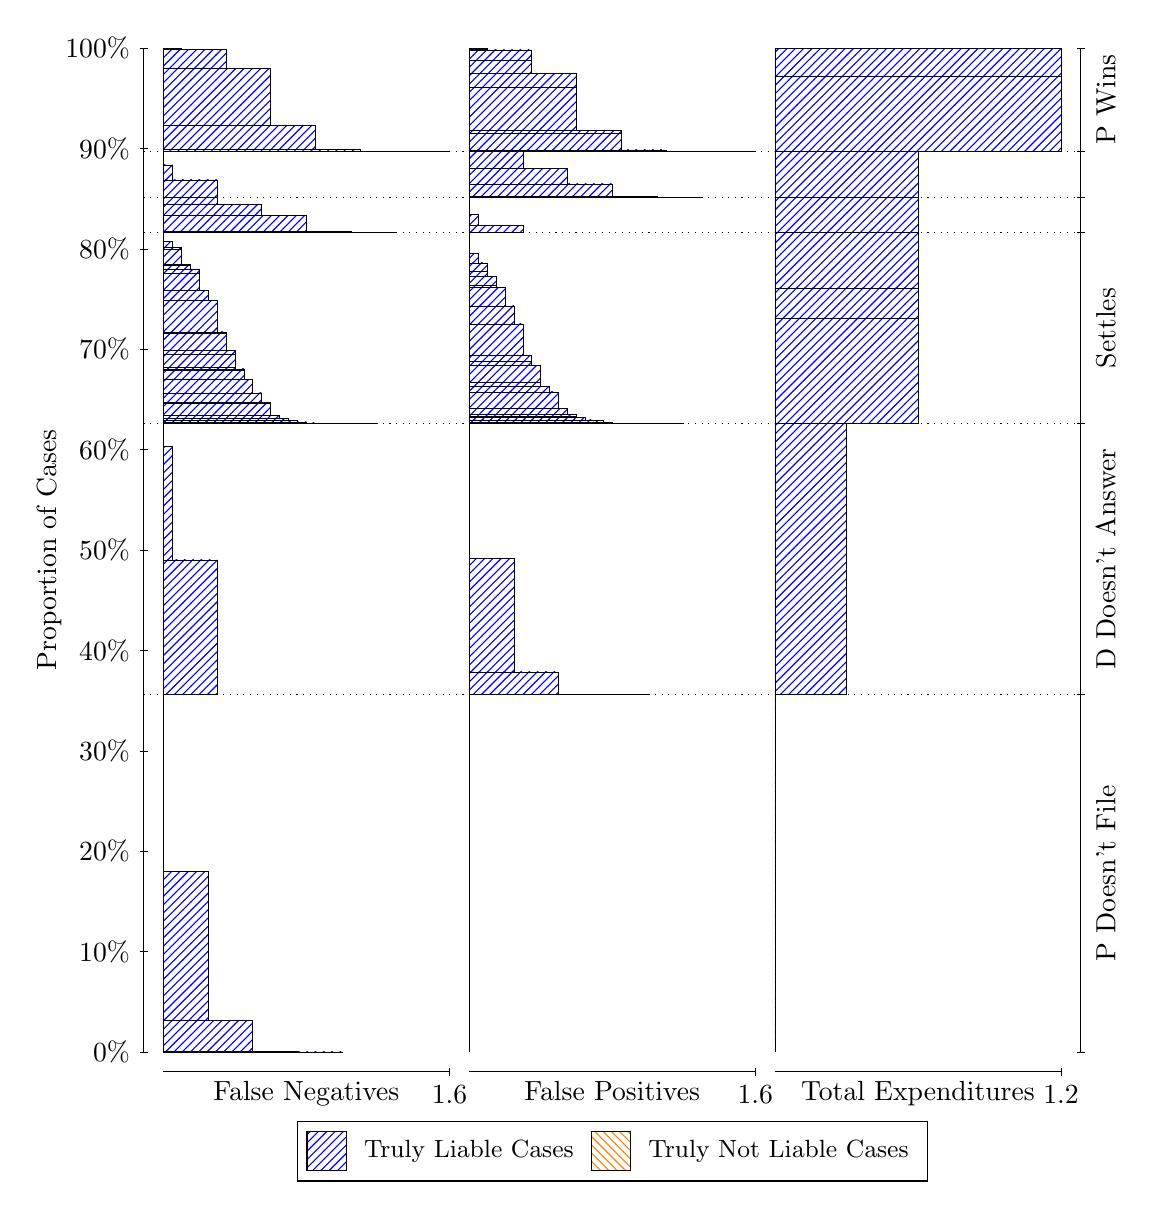
\begin{tikzpicture}
\draw[black, very thin] (1.5,1.75) -- (1.5,14.5);
\node[rotate=90, anchor=center] at (0.3, 8.125) {Proportion of Cases};
\draw[black, very thin] (1.45,1.75) -- (1.55,1.75);
\node[anchor=east] at (1.45, 1.75) {0\%};
\draw[black, very thin] (1.45,3.025) -- (1.55,3.025);
\node[anchor=east] at (1.45, 3.025) {10\%};
\draw[black, very thin] (1.45,4.3) -- (1.55,4.3);
\node[anchor=east] at (1.45, 4.3) {20\%};
\draw[black, very thin] (1.45,5.575) -- (1.55,5.575);
\node[anchor=east] at (1.45, 5.575) {30\%};
\draw[black, very thin] (1.45,6.85) -- (1.55,6.85);
\node[anchor=east] at (1.45, 6.85) {40\%};
\draw[black, very thin] (1.45,8.125) -- (1.55,8.125);
\node[anchor=east] at (1.45, 8.125) {50\%};
\draw[black, very thin] (1.45,9.4) -- (1.55,9.4);
\node[anchor=east] at (1.45, 9.4) {60\%};
\draw[black, very thin] (1.45,10.675) -- (1.55,10.675);
\node[anchor=east] at (1.45, 10.675) {70\%};
\draw[black, very thin] (1.45,11.95) -- (1.55,11.95);
\node[anchor=east] at (1.45, 11.95) {80\%};
\draw[black, very thin] (1.45,13.225) -- (1.55,13.225);
\node[anchor=east] at (1.45, 13.225) {90\%};
\draw[black, very thin] (1.45,14.5) -- (1.55,14.5);
\node[anchor=east] at (1.45, 14.5) {100\%};

\draw[black, very thin] (13.4,1.75) -- (13.4,14.5);
\draw[black, very thin] (13.35,1.75) -- (13.45,1.75);
\node[anchor=west] at (13.35, 1.75) {};
\draw[black, very thin] (13.35,6.287) -- (13.45,6.287);
\node[anchor=west] at (13.35, 6.287) {};
\draw[black, very thin] (13.35,9.7321) -- (13.45,9.7321);
\node[anchor=west] at (13.35, 9.7321) {};
\draw[black, very thin] (13.35,12.159) -- (13.45,12.159);
\node[anchor=west] at (13.35, 12.159) {};
\draw[black, very thin] (13.35,12.603) -- (13.45,12.603);
\node[anchor=west] at (13.35, 12.603) {};
\draw[black, very thin] (13.35,13.189) -- (13.45,13.189);
\node[anchor=west] at (13.35, 13.189) {};
\draw[black, very thin] (13.35,14.5) -- (13.45,14.5);
\node[anchor=west] at (13.35, 14.5) {};

\draw[black, very thin, pattern color=blue, pattern=north east lines] (1.75,1.75) rectangle (4.0208,1.7501);
\draw[black, very thin, pattern color=blue, pattern=north east lines] (1.75,1.7501) rectangle (3.4531,1.7603);
\draw[black, very thin, pattern color=blue, pattern=north east lines] (1.75,1.7603) rectangle (2.8854,2.1481);
\draw[black, very thin, pattern color=blue, pattern=north east lines] (1.75,2.1481) rectangle (2.3177,4.0445);
\draw[black, very thin, pattern color=orange, pattern=north west lines] (1.75,4.0445) rectangle (1.75,4.0445);
\draw[black, very thin, pattern color=blue, pattern=north east lines] (1.75,4.0445) rectangle (1.75,6.287);
\draw[black, very thin, pattern color=blue, pattern=north east lines] (1.75,6.287) rectangle (2.4312,7.9998);
\draw[black, very thin, pattern color=blue, pattern=north east lines] (1.75,7.9998) rectangle (1.8635,9.4415);
\draw[black, very thin, pattern color=orange, pattern=north west lines] (1.75,9.4415) rectangle (1.75,9.4415);
\draw[black, very thin, pattern color=blue, pattern=north east lines] (1.75,9.4415) rectangle (1.75,9.7321);
\draw[black, very thin, pattern color=blue, pattern=north east lines] (1.75,9.7321) rectangle (4.475,9.7321);
\draw[black, very thin, pattern color=blue, pattern=north east lines] (1.75,9.7321) rectangle (4.2479,9.7321);
\draw[black, very thin, pattern color=blue, pattern=north east lines] (1.75,9.7321) rectangle (4.0208,9.7346);
\draw[black, very thin, pattern color=blue, pattern=north east lines] (1.75,9.7346) rectangle (3.9073,9.7353);
\draw[black, very thin, pattern color=blue, pattern=north east lines] (1.75,9.7353) rectangle (3.7937,9.7353);
\draw[black, very thin, pattern color=blue, pattern=north east lines] (1.75,9.7353) rectangle (3.7937,9.7378);
\draw[black, very thin, pattern color=blue, pattern=north east lines] (1.75,9.7378) rectangle (3.6802,9.7388);
\draw[black, very thin, pattern color=blue, pattern=north east lines] (1.75,9.7388) rectangle (3.5667,9.7521);
\draw[black, very thin, pattern color=blue, pattern=north east lines] (1.75,9.7521) rectangle (3.4531,9.7724);
\draw[black, very thin, pattern color=blue, pattern=north east lines] (1.75,9.7724) rectangle (3.3396,9.797);
\draw[black, very thin, pattern color=blue, pattern=north east lines] (1.75,9.797) rectangle (3.226,9.7992);
\draw[black, very thin, pattern color=blue, pattern=north east lines] (1.75,9.7992) rectangle (3.226,9.8299);
\draw[black, very thin, pattern color=blue, pattern=north east lines] (1.75,9.8299) rectangle (3.1125,9.9894);
\draw[black, very thin, pattern color=blue, pattern=north east lines] (1.75,9.9894) rectangle (3.1125,10.002);
\draw[black, very thin, pattern color=blue, pattern=north east lines] (1.75,10.002) rectangle (2.999,10.121);
\draw[black, very thin, pattern color=blue, pattern=north east lines] (1.75,10.121) rectangle (2.8854,10.293);
\draw[black, very thin, pattern color=blue, pattern=north east lines] (1.75,10.293) rectangle (2.7719,10.409);
\draw[black, very thin, pattern color=blue, pattern=north east lines] (1.75,10.409) rectangle (2.7719,10.426);
\draw[black, very thin, pattern color=blue, pattern=north east lines] (1.75,10.426) rectangle (2.6583,10.444);
\draw[black, very thin, pattern color=blue, pattern=north east lines] (1.75,10.444) rectangle (2.6583,10.608);
\draw[black, very thin, pattern color=blue, pattern=north east lines] (1.75,10.608) rectangle (2.6583,10.665);
\draw[black, very thin, pattern color=blue, pattern=north east lines] (1.75,10.665) rectangle (2.5448,10.873);
\draw[black, very thin, pattern color=blue, pattern=north east lines] (1.75,10.873) rectangle (2.5448,10.894);
\draw[black, very thin, pattern color=blue, pattern=north east lines] (1.75,10.894) rectangle (2.4312,11.299);
\draw[black, very thin, pattern color=blue, pattern=north east lines] (1.75,11.299) rectangle (2.3177,11.422);
\draw[black, very thin, pattern color=blue, pattern=north east lines] (1.75,11.422) rectangle (2.2042,11.634);
\draw[black, very thin, pattern color=blue, pattern=north east lines] (1.75,11.634) rectangle (2.2042,11.685);
\draw[black, very thin, pattern color=blue, pattern=north east lines] (1.75,11.685) rectangle (2.0906,11.695);
\draw[black, very thin, pattern color=blue, pattern=north east lines] (1.75,11.695) rectangle (2.0906,11.737);
\draw[black, very thin, pattern color=blue, pattern=north east lines] (1.75,11.737) rectangle (2.0906,11.757);
\draw[black, very thin, pattern color=blue, pattern=north east lines] (1.75,11.757) rectangle (1.9771,11.95);
\draw[black, very thin, pattern color=blue, pattern=north east lines] (1.75,11.95) rectangle (1.9771,11.966);
\draw[black, very thin, pattern color=blue, pattern=north east lines] (1.75,11.966) rectangle (1.8635,12.044);
\draw[black, very thin, pattern color=orange, pattern=north west lines] (1.75,12.044) rectangle (1.75,12.044);
\draw[black, very thin, pattern color=blue, pattern=north east lines] (1.75,12.044) rectangle (1.75,12.159);
\draw[black, very thin, pattern color=blue, pattern=north east lines] (1.75,12.159) rectangle (4.7021,12.159);
\draw[black, very thin, pattern color=blue, pattern=north east lines] (1.75,12.159) rectangle (4.1344,12.176);
\draw[black, very thin, pattern color=blue, pattern=north east lines] (1.75,12.176) rectangle (3.5667,12.372);
\draw[black, very thin, pattern color=blue, pattern=north east lines] (1.75,12.372) rectangle (2.999,12.514);
\draw[black, very thin, pattern color=blue, pattern=north east lines] (1.75,12.514) rectangle (2.4312,12.603);
\draw[black, very thin, pattern color=orange, pattern=north west lines] (1.75,12.603) rectangle (1.75,12.603);
\draw[black, very thin, pattern color=blue, pattern=north east lines] (1.75,12.603) rectangle (2.4312,12.824);
\draw[black, very thin, pattern color=blue, pattern=north east lines] (1.75,12.824) rectangle (1.8635,13.017);
\draw[black, very thin, pattern color=orange, pattern=north west lines] (1.75,13.017) rectangle (1.75,13.017);
\draw[black, very thin, pattern color=blue, pattern=north east lines] (1.75,13.017) rectangle (1.75,13.189);
\draw[black, very thin, pattern color=blue, pattern=north east lines] (1.75,13.189) rectangle (5.3833,13.189);
\draw[black, very thin, pattern color=blue, pattern=north east lines] (1.75,13.189) rectangle (4.8156,13.19);
\draw[black, very thin, pattern color=blue, pattern=north east lines] (1.75,13.19) rectangle (4.2479,13.215);
\draw[black, very thin, pattern color=blue, pattern=north east lines] (1.75,13.215) rectangle (3.6802,13.515);
\draw[black, very thin, pattern color=blue, pattern=north east lines] (1.75,13.515) rectangle (3.1125,14.24);
\draw[black, very thin, pattern color=blue, pattern=north east lines] (1.75,14.24) rectangle (2.5448,14.483);
\draw[black, very thin, pattern color=blue, pattern=north east lines] (1.75,14.483) rectangle (1.9771,14.5);
\draw[black, very thin, pattern color=orange, pattern=north west lines] (1.75,14.5) rectangle (1.75,14.5);
\draw[black, very thin, pattern color=blue, pattern=north east lines] (1.75,14.5) rectangle (1.75,14.5);
\draw[black, very thin, pattern color=orange, pattern=north west lines] (5.6333,1.75) rectangle (5.6333,1.75);
\draw[black, very thin, pattern color=blue, pattern=north east lines] (5.6333,1.75) rectangle (5.6333,6.287);
\draw[black, very thin, pattern color=orange, pattern=north west lines] (5.6333,6.287) rectangle (7.9042,6.287);
\draw[black, very thin, pattern color=blue, pattern=north east lines] (5.6333,6.287) rectangle (7.9042,6.2871);
\draw[black, very thin, pattern color=blue, pattern=north east lines] (5.6333,6.2871) rectangle (7.3365,6.2916);
\draw[black, very thin, pattern color=blue, pattern=north east lines] (5.6333,6.2916) rectangle (6.7687,6.5776);
\draw[black, very thin, pattern color=blue, pattern=north east lines] (5.6333,6.5776) rectangle (6.201,8.0193);
\draw[black, very thin, pattern color=blue, pattern=north east lines] (5.6333,8.0193) rectangle (5.6333,9.7321);
\draw[black, very thin, pattern color=orange, pattern=north west lines] (5.6333,9.7321) rectangle (8.3583,9.7321);
\draw[black, very thin, pattern color=blue, pattern=north east lines] (5.6333,9.7321) rectangle (8.3583,9.7321);
\draw[black, very thin, pattern color=orange, pattern=north west lines] (5.6333,9.7321) rectangle (8.1313,9.7321);
\draw[black, very thin, pattern color=blue, pattern=north east lines] (5.6333,9.7321) rectangle (8.1313,9.7322);
\draw[black, very thin, pattern color=orange, pattern=north west lines] (5.6333,9.7322) rectangle (7.9042,9.7322);
\draw[black, very thin, pattern color=blue, pattern=north east lines] (5.6333,9.7322) rectangle (7.9042,9.7339);
\draw[black, very thin, pattern color=blue, pattern=north east lines] (5.6333,9.7339) rectangle (7.7906,9.7342);
\draw[black, very thin, pattern color=orange, pattern=north west lines] (5.6333,9.7342) rectangle (7.6771,9.7342);
\draw[black, very thin, pattern color=blue, pattern=north east lines] (5.6333,9.7342) rectangle (7.6771,9.736);
\draw[black, very thin, pattern color=blue, pattern=north east lines] (5.6333,9.736) rectangle (7.5635,9.7372);
\draw[black, very thin, pattern color=orange, pattern=north west lines] (5.6333,9.7372) rectangle (7.45,9.7372);
\draw[black, very thin, pattern color=blue, pattern=north east lines] (5.6333,9.7372) rectangle (7.45,9.7423);
\draw[black, very thin, pattern color=blue, pattern=north east lines] (5.6333,9.7423) rectangle (7.3365,9.7692);
\draw[black, very thin, pattern color=orange, pattern=north west lines] (5.6333,9.7692) rectangle (7.2229,9.7692);
\draw[black, very thin, pattern color=blue, pattern=north east lines] (5.6333,9.7692) rectangle (7.2229,9.7771);
\draw[black, very thin, pattern color=blue, pattern=north east lines] (5.6333,9.7771) rectangle (7.1094,9.8107);
\draw[black, very thin, pattern color=blue, pattern=north east lines] (5.6333,9.8107) rectangle (6.9958,9.826);
\draw[black, very thin, pattern color=orange, pattern=north west lines] (5.6333,9.826) rectangle (6.9958,9.826);
\draw[black, very thin, pattern color=blue, pattern=north east lines] (5.6333,9.826) rectangle (6.9958,9.8473);
\draw[black, very thin, pattern color=blue, pattern=north east lines] (5.6333,9.8473) rectangle (6.8823,9.9251);
\draw[black, very thin, pattern color=orange, pattern=north west lines] (5.6333,9.9251) rectangle (6.7687,9.9251);
\draw[black, very thin, pattern color=blue, pattern=north east lines] (5.6333,9.9251) rectangle (6.7687,10.134);
\draw[black, very thin, pattern color=blue, pattern=north east lines] (5.6333,10.134) rectangle (6.6552,10.206);
\draw[black, very thin, pattern color=orange, pattern=north west lines] (5.6333,10.206) rectangle (6.5417,10.206);
\draw[black, very thin, pattern color=blue, pattern=north east lines] (5.6333,10.206) rectangle (6.5417,10.257);
\draw[black, very thin, pattern color=blue, pattern=north east lines] (5.6333,10.257) rectangle (6.5417,10.469);
\draw[black, very thin, pattern color=blue, pattern=north east lines] (5.6333,10.469) rectangle (6.4281,10.52);
\draw[black, very thin, pattern color=blue, pattern=north east lines] (5.6333,10.52) rectangle (6.4281,10.592);
\draw[black, very thin, pattern color=blue, pattern=north east lines] (5.6333,10.592) rectangle (6.3146,10.997);
\draw[black, very thin, pattern color=blue, pattern=north east lines] (5.6333,10.997) rectangle (6.201,11.226);
\draw[black, very thin, pattern color=blue, pattern=north east lines] (5.6333,11.226) rectangle (6.0875,11.464);
\draw[black, very thin, pattern color=blue, pattern=north east lines] (5.6333,11.464) rectangle (5.974,11.482);
\draw[black, very thin, pattern color=blue, pattern=north east lines] (5.6333,11.482) rectangle (5.974,11.598);
\draw[black, very thin, pattern color=blue, pattern=north east lines] (5.6333,11.598) rectangle (5.8604,11.659);
\draw[black, very thin, pattern color=blue, pattern=north east lines] (5.6333,11.659) rectangle (5.8604,11.77);
\draw[black, very thin, pattern color=blue, pattern=north east lines] (5.6333,11.77) rectangle (5.7469,11.888);
\draw[black, very thin, pattern color=blue, pattern=north east lines] (5.6333,11.888) rectangle (5.6333,12.159);
\draw[black, very thin, pattern color=orange, pattern=north west lines] (5.6333,12.159) rectangle (6.3146,12.159);
\draw[black, very thin, pattern color=blue, pattern=north east lines] (5.6333,12.159) rectangle (6.3146,12.248);
\draw[black, very thin, pattern color=blue, pattern=north east lines] (5.6333,12.248) rectangle (5.7469,12.39);
\draw[black, very thin, pattern color=blue, pattern=north east lines] (5.6333,12.39) rectangle (5.6333,12.603);
\draw[black, very thin, pattern color=orange, pattern=north west lines] (5.6333,12.603) rectangle (8.5854,12.603);
\draw[black, very thin, pattern color=blue, pattern=north east lines] (5.6333,12.603) rectangle (8.5854,12.604);
\draw[black, very thin, pattern color=blue, pattern=north east lines] (5.6333,12.604) rectangle (8.0177,12.616);
\draw[black, very thin, pattern color=blue, pattern=north east lines] (5.6333,12.616) rectangle (7.45,12.775);
\draw[black, very thin, pattern color=blue, pattern=north east lines] (5.6333,12.775) rectangle (6.8823,12.969);
\draw[black, very thin, pattern color=blue, pattern=north east lines] (5.6333,12.969) rectangle (6.3146,13.189);
\draw[black, very thin, pattern color=orange, pattern=north west lines] (5.6333,13.189) rectangle (9.2667,13.189);
\draw[black, very thin, pattern color=blue, pattern=north east lines] (5.6333,13.189) rectangle (9.2667,13.189);
\draw[black, very thin, pattern color=orange, pattern=north west lines] (5.6333,13.189) rectangle (8.699,13.189);
\draw[black, very thin, pattern color=blue, pattern=north east lines] (5.6333,13.189) rectangle (8.699,13.19);
\draw[black, very thin, pattern color=orange, pattern=north west lines] (5.6333,13.19) rectangle (8.1313,13.19);
\draw[black, very thin, pattern color=blue, pattern=north east lines] (5.6333,13.19) rectangle (8.1313,13.206);
\draw[black, very thin, pattern color=blue, pattern=north east lines] (5.6333,13.206) rectangle (7.5635,13.414);
\draw[black, very thin, pattern color=orange, pattern=north west lines] (5.6333,13.414) rectangle (7.5635,13.414);
\draw[black, very thin, pattern color=blue, pattern=north east lines] (5.6333,13.414) rectangle (7.5635,13.45);
\draw[black, very thin, pattern color=blue, pattern=north east lines] (5.6333,13.45) rectangle (6.9958,14.001);
\draw[black, very thin, pattern color=orange, pattern=north west lines] (5.6333,14.001) rectangle (6.9958,14.001);
\draw[black, very thin, pattern color=blue, pattern=north east lines] (5.6333,14.001) rectangle (6.9958,14.174);
\draw[black, very thin, pattern color=blue, pattern=north east lines] (5.6333,14.174) rectangle (6.4281,14.342);
\draw[black, very thin, pattern color=blue, pattern=north east lines] (5.6333,14.342) rectangle (6.4281,14.475);
\draw[black, very thin, pattern color=blue, pattern=north east lines] (5.6333,14.475) rectangle (5.8604,14.484);
\draw[black, very thin, pattern color=blue, pattern=north east lines] (5.6333,14.484) rectangle (5.8604,14.5);
\draw[black, very thin, pattern color=blue, pattern=north east lines] (5.6333,14.5) rectangle (5.6333,14.5);
\draw[black, very thin, pattern color=orange, pattern=north west lines] (9.5167,1.75) rectangle (9.5167,1.75);
\draw[black, very thin, pattern color=blue, pattern=north east lines] (9.5167,1.75) rectangle (9.5167,6.287);
\draw[black, very thin, pattern color=orange, pattern=north west lines] (9.5167,6.287) rectangle (10.425,6.287);
\draw[black, very thin, pattern color=blue, pattern=north east lines] (9.5167,6.287) rectangle (10.425,9.7321);
\draw[black, very thin, pattern color=orange, pattern=north west lines] (9.5167,9.7321) rectangle (11.333,9.7321);
\draw[black, very thin, pattern color=blue, pattern=north east lines] (9.5167,9.7321) rectangle (11.333,11.069);
\draw[black, very thin, pattern color=orange, pattern=north west lines] (9.5167,11.069) rectangle (11.333,11.069);
\draw[black, very thin, pattern color=blue, pattern=north east lines] (9.5167,11.069) rectangle (11.333,11.453);
\draw[black, very thin, pattern color=orange, pattern=north west lines] (9.5167,11.453) rectangle (11.333,11.453);
\draw[black, very thin, pattern color=blue, pattern=north east lines] (9.5167,11.453) rectangle (11.333,12.159);
\draw[black, very thin, pattern color=orange, pattern=north west lines] (9.5167,12.159) rectangle (11.333,12.159);
\draw[black, very thin, pattern color=blue, pattern=north east lines] (9.5167,12.159) rectangle (11.333,12.603);
\draw[black, very thin, pattern color=orange, pattern=north west lines] (9.5167,12.603) rectangle (11.333,12.603);
\draw[black, very thin, pattern color=blue, pattern=north east lines] (9.5167,12.603) rectangle (11.333,13.189);
\draw[black, very thin, pattern color=orange, pattern=north west lines] (9.5167,13.189) rectangle (13.15,13.189);
\draw[black, very thin, pattern color=blue, pattern=north east lines] (9.5167,13.189) rectangle (13.15,14.142);
\draw[black, very thin, pattern color=orange, pattern=north west lines] (9.5167,14.142) rectangle (13.15,14.142);
\draw[black, very thin, pattern color=blue, pattern=north east lines] (9.5167,14.142) rectangle (13.15,14.5);
\draw[black, dotted] (1.5,6.287) -- (13.4,6.287);
\draw[black, dotted] (1.5,9.7321) -- (13.4,9.7321);
\draw[black, dotted] (1.5,12.159) -- (13.4,12.159);
\draw[black, dotted] (1.5,12.603) -- (13.4,12.603);
\draw[black, dotted] (1.5,13.189) -- (13.4,13.189);
\draw[black, very thin] (1.75,1.5) -- (5.3833,1.5);
\node[anchor=north] at (3.5667, 1.5) {False Negatives};
\draw[black, very thin] (5.3833,1.45) -- (5.3833,1.55);
\node[anchor=north] at (5.3833, 1.45) {1.6};

\draw[black, very thin] (5.6333,1.5) -- (9.2667,1.5);
\node[anchor=north] at (7.45, 1.5) {False Positives};
\draw[black, very thin] (9.2667,1.45) -- (9.2667,1.55);
\node[anchor=north] at (9.2667, 1.45) {1.6};

\draw[black, very thin] (9.5167,1.5) -- (13.15,1.5);
\node[anchor=north] at (11.333, 1.5) {Total Expenditures};
\draw[black, very thin] (13.15,1.45) -- (13.15,1.55);
\node[anchor=north] at (13.15, 1.45) {1.2};

\node[black, centered, rotate=90] at (13.72, 4.0185) {P Doesn't File};
\node[black, centered, rotate=90] at (13.72, 8.0096) {D Doesn't Answer};
\node[black, centered, rotate=90] at (13.72, 10.945) {Settles};


\node[black, centered, rotate=90] at (13.72, 13.845) {P Wins};

\draw (7.449999999999999,1.5) node[draw=none] (baseCoordinate) {};
\begin{scope}[align=center]
        \matrix[scale=0.5, draw=black, below=0.5cm of baseCoordinate, nodes={draw}, column sep=0.1cm]{
            \node[rectangle, draw, minimum width=0.5cm, minimum height=0.5cm, pattern=north east lines, pattern color=blue] {}; &
            \node[draw=none, font=\small] (B) {Truly Liable Cases}; &
            \node[rectangle, draw, minimum width=0.5cm, minimum height=0.5cm, pattern=north west lines, pattern color=orange] {}; &
            \node[draw=none, font=\small] (B) {Truly Not Liable Cases}; \\
            };
\end{scope}

\end{tikzpicture}
\end{document}